
\begin{figure}[H]
  {
    \setlength{\tabcolsep}{3.0pt}
    \setlength\cmidrulewidth{\heavyrulewidth} % Make cmidrule = 
    \begin{adjustbox}{height=5cm,center}
      \footnotesize
      \begin{tabular}{ll}

        \makecell[l]{
\icode{.BYTE \$00}\\
\icode{.BYTE \$00}
} & \makecell[l]{
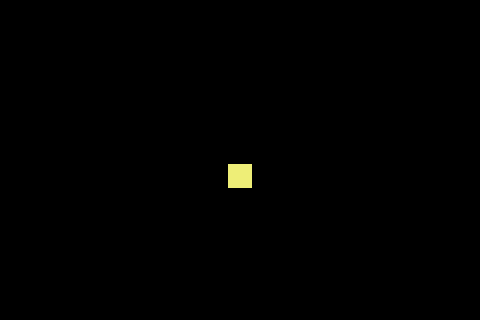
\includegraphics[width=1.3cm]{src/patterns/pixels/pixel_pattern10_0.png}%
} \\
        \midrule

        \makecell[l]{
\icode{.BYTE \$00,\$FD,\$03}\\
\icode{.BYTE \$00,\$00,\$00}
} & \makecell[l]{
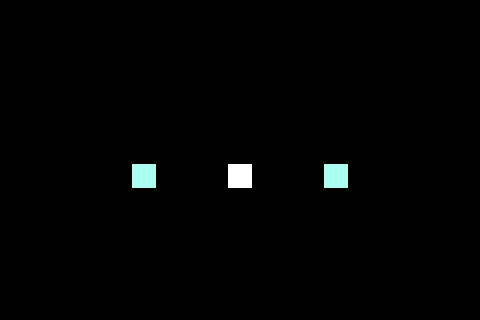
\includegraphics[width=1.3cm]{src/patterns/pixels/pixel_pattern10_1.png}%
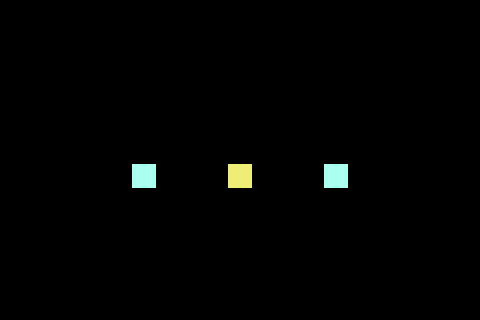
\includegraphics[width=1.3cm]{src/patterns/pixels/pixel_pattern10_2.png}%
} \\
        \midrule

        \makecell[l]{
\icode{.BYTE \$00,\$F9,\$07}\\
\icode{.BYTE \$00,\$00,\$00}
} & \makecell[l]{
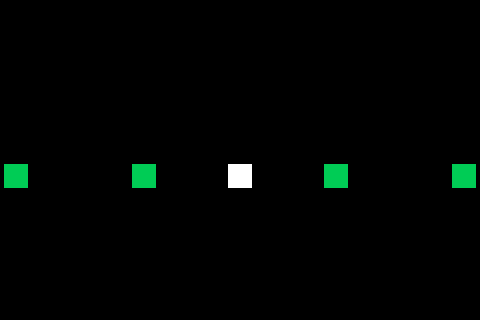
\includegraphics[width=1.3cm]{src/patterns/pixels/pixel_pattern10_3.png}%
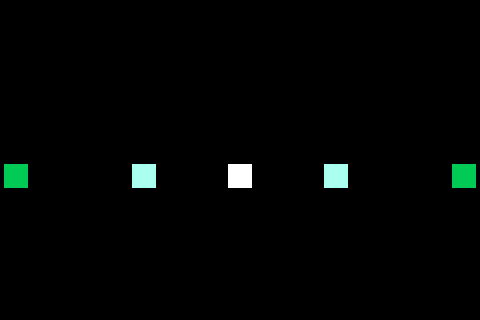
\includegraphics[width=1.3cm]{src/patterns/pixels/pixel_pattern10_4.png}%
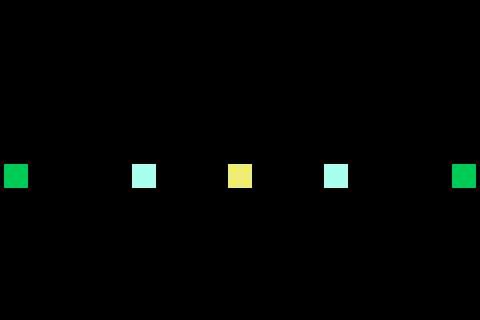
\includegraphics[width=1.3cm]{src/patterns/pixels/pixel_pattern10_5.png}%
} \\
        \midrule

        \makecell[l]{
\icode{.BYTE \$00,\$FB,\$05}\\
\icode{.BYTE \$00,\$FD,\$FD}
} & \makecell[l]{
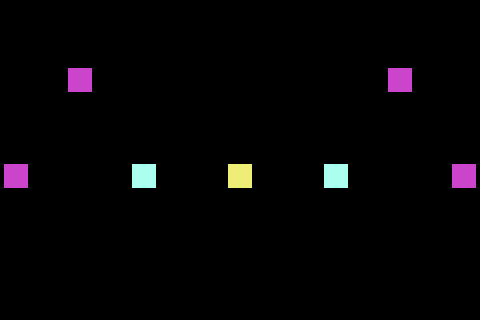
\includegraphics[width=1.3cm]{src/patterns/pixels/pixel_pattern10_6.png}%
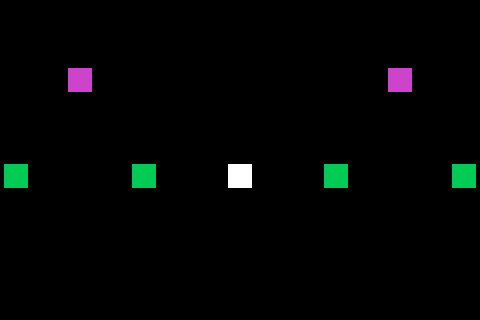
\includegraphics[width=1.3cm]{src/patterns/pixels/pixel_pattern10_7.png}%
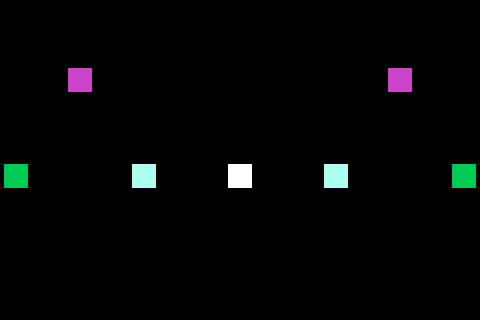
\includegraphics[width=1.3cm]{src/patterns/pixels/pixel_pattern10_8.png}%
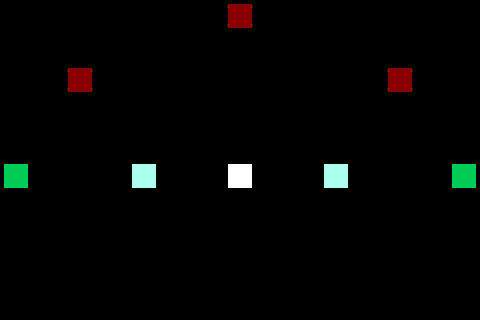
\includegraphics[width=1.3cm]{src/patterns/pixels/pixel_pattern10_9.png}%
} \\
        \midrule

        \makecell[l]{
\icode{.BYTE \$00,\$00}\\
\icode{.BYTE \$00,\$FB}
} & \makecell[l]{
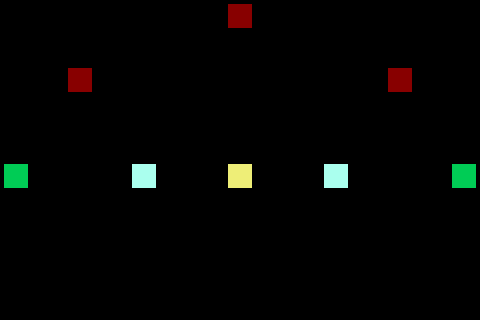
\includegraphics[width=1.3cm]{src/patterns/pixels/pixel_pattern10_10.png}%
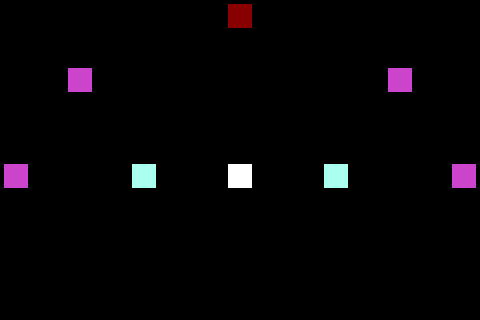
\includegraphics[width=1.3cm]{src/patterns/pixels/pixel_pattern10_11.png}%
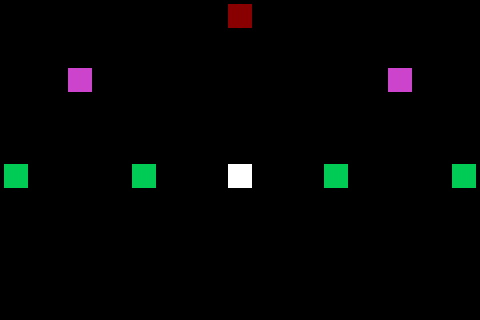
\includegraphics[width=1.3cm]{src/patterns/pixels/pixel_pattern10_12.png}%
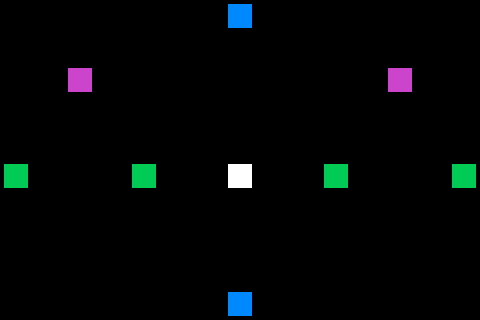
\includegraphics[width=1.3cm]{src/patterns/pixels/pixel_pattern10_13.png}%
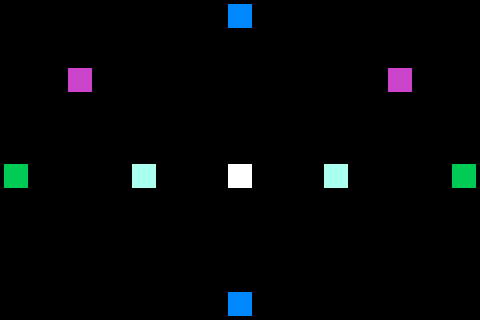
\includegraphics[width=1.3cm]{src/patterns/pixels/pixel_pattern10_14.png}%
} \\
        \midrule

        \makecell[l]{
\icode{.BYTE \$00,\$00}\\
\icode{.BYTE \$00,\$04}
} & \makecell[l]{
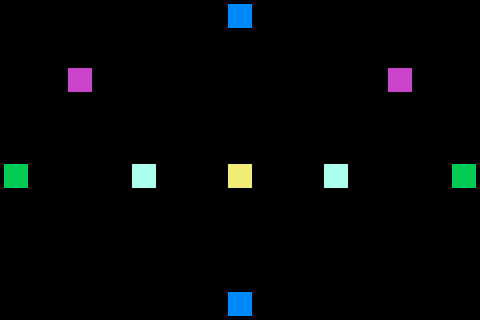
\includegraphics[width=1.3cm]{src/patterns/pixels/pixel_pattern10_15.png}%
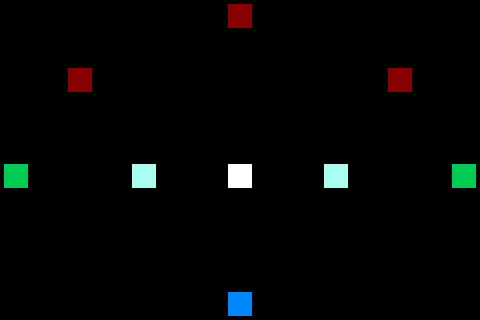
\includegraphics[width=1.3cm]{src/patterns/pixels/pixel_pattern10_16.png}%
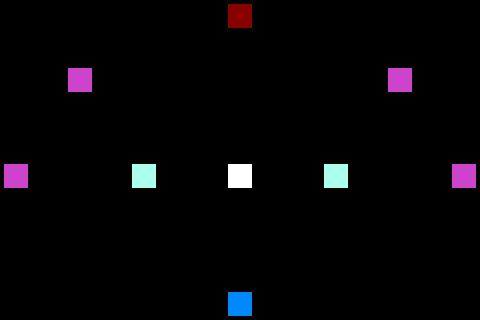
\includegraphics[width=1.3cm]{src/patterns/pixels/pixel_pattern10_17.png}%
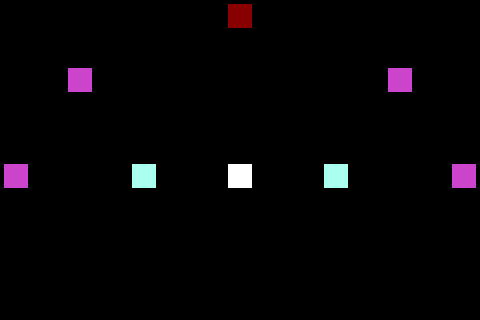
\includegraphics[width=1.3cm]{src/patterns/pixels/pixel_pattern10_18.png}%
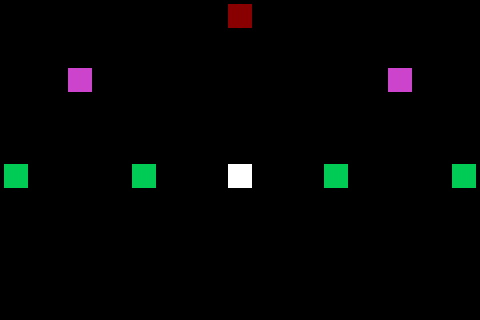
\includegraphics[width=1.3cm]{src/patterns/pixels/pixel_pattern10_19.png}%
} \\
        \midrule

        \makecell[l]{
\icode{.BYTE \$00}\\
\icode{.BYTE \$00}
} & \makecell[l]{
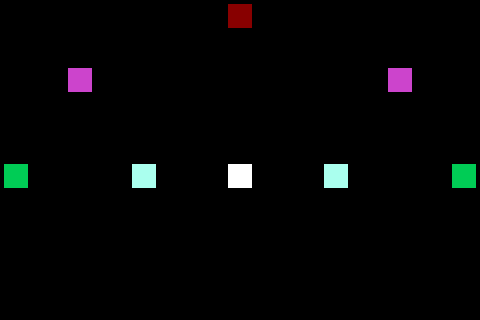
\includegraphics[width=1.3cm]{src/patterns/pixels/pixel_pattern10_20.png}%
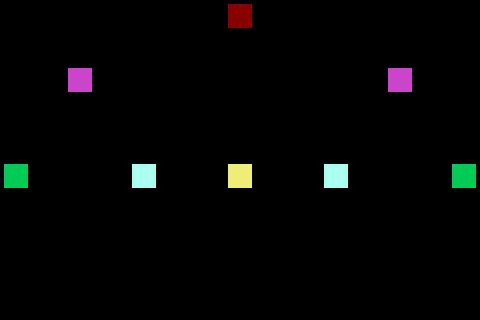
\includegraphics[width=1.3cm]{src/patterns/pixels/pixel_pattern10_21.png}%
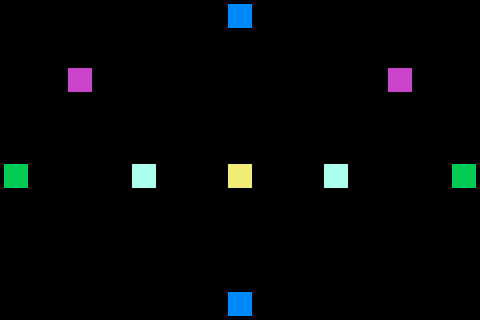
\includegraphics[width=1.3cm]{src/patterns/pixels/pixel_pattern10_22.png}%
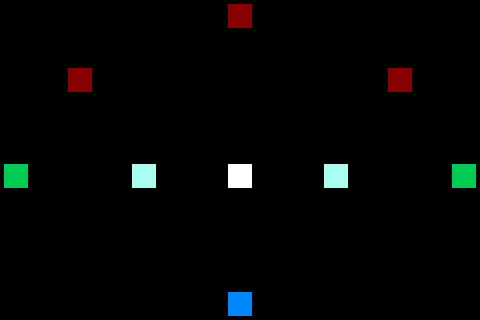
\includegraphics[width=1.3cm]{src/patterns/pixels/pixel_pattern10_23.png}%
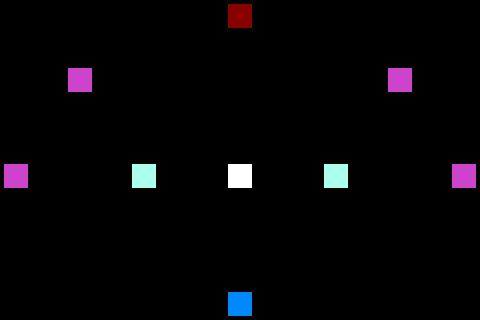
\includegraphics[width=1.3cm]{src/patterns/pixels/pixel_pattern10_24.png}%
} \\
        \midrule

        \makecell[l]{
\icode{.BYTE \$FE,\$02}\\
\icode{.BYTE \$FC,\$FC}
} & \makecell[l]{
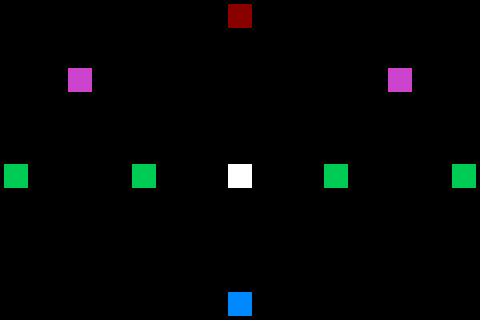
\includegraphics[width=1.3cm]{src/patterns/pixels/pixel_pattern10_25.png}%
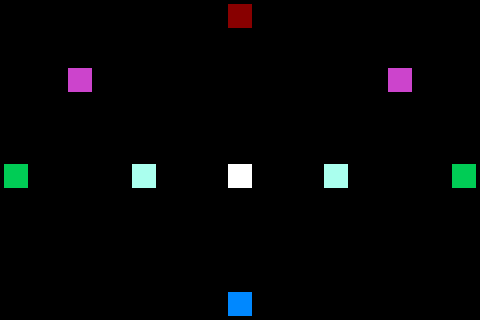
\includegraphics[width=1.3cm]{src/patterns/pixels/pixel_pattern10_26.png}%
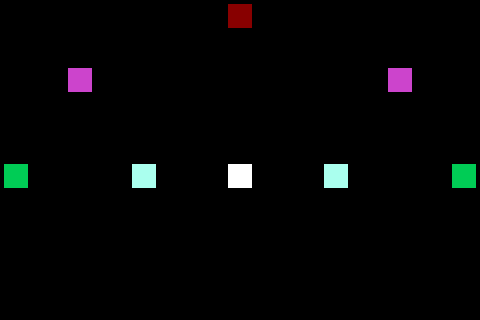
\includegraphics[width=1.3cm]{src/patterns/pixels/pixel_pattern10_27.png}%
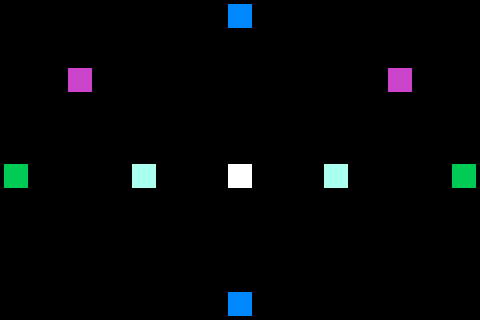
\includegraphics[width=1.3cm]{src/patterns/pixels/pixel_pattern10_28.png}%
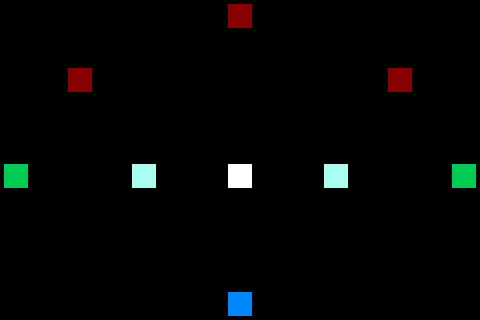
\includegraphics[width=1.3cm]{src/patterns/pixels/pixel_pattern10_29.png}%
} \\
        \midrule

        \makecell[l]{
\icode{.BYTE \$00}\\
\icode{.BYTE \$00}
} & \makecell[l]{
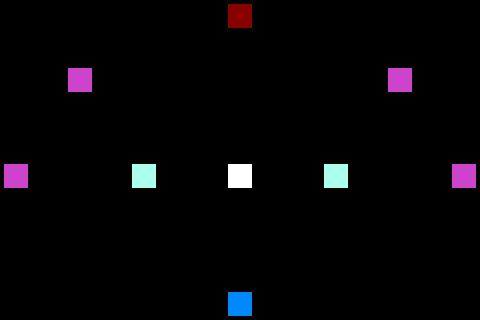
\includegraphics[width=1.3cm]{src/patterns/pixels/pixel_pattern10_30.png}%
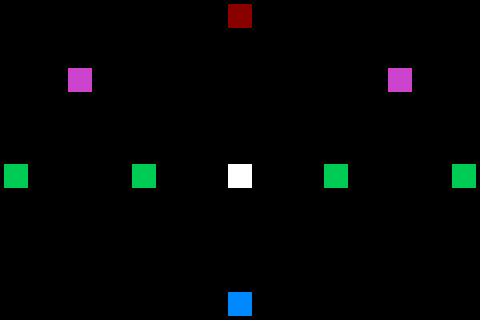
\includegraphics[width=1.3cm]{src/patterns/pixels/pixel_pattern10_31.png}%
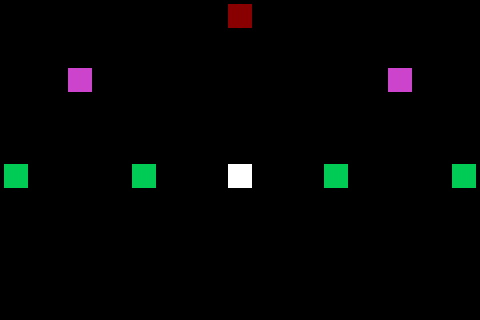
\includegraphics[width=1.3cm]{src/patterns/pixels/pixel_pattern10_32.png}%
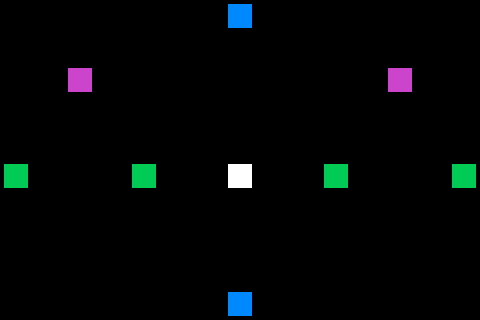
\includegraphics[width=1.3cm]{src/patterns/pixels/pixel_pattern10_33.png}%
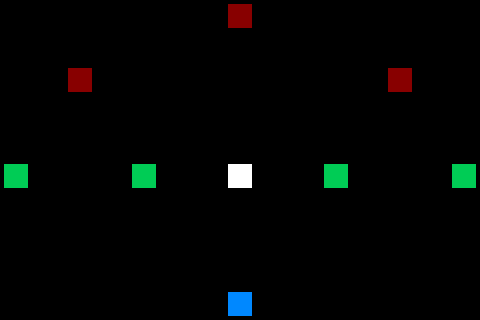
\includegraphics[width=1.3cm]{src/patterns/pixels/pixel_pattern10_34.png}%
} \\
        \midrule

      \end{tabular}
    \end{adjustbox}
  }\caption{The purpose of each of the oscillator values.}
\end{figure}
